\documentclass[journal]{IEEEtran}

\usepackage{xeCJK} % CJK语言环境,使用XeLaTex进行编译
\usepackage{authblk} % 对应中文部分的作者机构特殊语法

% 将 authblk 包中的作者连词 and 替换为中文逗号
\renewcommand*{\Authsep}{,}
\renewcommand*{\Authand}{,}
\renewcommand*{\Authands}{,}

\setlength{\parindent}{2em} %2em代表首行缩进两个字符

%行间距
\usepackage{setspace} % 用于设置行间距

\onehalfspacing%设置1.5倍行距
%字号
\fontsize{22pt}{\baselineskip}{\selectfont}

%设置英文正文字体
\setmainfont{Times New Roman}
\usepackage{fontspec}

%图片
\usepackage{graphicx} %插入图片的宏包
\usepackage{float} %设置图片浮动位置的宏包
\usepackage{subfigure} %插入多图时用子图显示的宏包

\usepackage[justification=centering]{caption}

%段间距
\setlength{\parskip}{1pt}

% 设置图注编号为图1-1格式
\captionsetup[figure]{labelformat=simple, labelsep=quad, font={small, singlespacing}, justification=raggedright}

\captionsetup[table]{labelformat=simple, labelsep=quad, font={small, singlespacing}, justification=raggedright}

\usepackage{amsmath}
\numberwithin{figure}{section}%关联图号和章节,应该是每一个section重置一下图号计数器
\renewcommand {\thefigure} {\arabic{section}-\arabic{figure}}%修改图号格式
\renewcommand\figurename{图} 

%引用
\usepackage{cite}

% correct bad hyphenation here
\hyphenation{op-tical net-works semi-conduc-tor}

\begin{document}

% paper title
\title{基于YOLOv8的头盔检测模型\\设计与实现}

\author{陈劭杰,郭昊,蔡明珠,刘政,黄俊毅,王晶昊,杨双菁,田睿朴,苗馨月% <-this % stops a space
\thanks{感谢电子科技大学机器学习课程闫老师与张老师的教学。}% <-this % stops a space
\thanks{2024年10月}}


% The paper headers
\markboth{Journal of \LaTeX\ Class Files,~Vol.~14, No.~8, October~2015}%
{Shell \MakeLowercase{\textit{et al.}}: 机器学习课程设计报告}


% make the title area
\maketitle

% As a general rule, do not put math, special symbols or citations
% in the abstract or keywords.
\begin{abstract}
	With the acceleration of industrial automation and urbanization, workplace safety issues have received increasing attention. Among various safety measures, the correct wearing of safety helmets is crucial for reducing head injuries. Therefore, developing an efficient and accurate helmet-wearing detection system is vital for improving safety at job sites. This paper proposes an improved model based on YOLOv8 for detecting whether individuals are wearing helmets. The model incorporates two key enhancements: first, a Transformer block replaces the bottleneck in the c2f module to enhance the model's ability to capture spatial features; second, the Convolutional Block Attention Module (CBAM) is integrated into the feature extraction process to further increase the model's focus on important areas and overall detection accuracy. Experimental results show that the modified model significantly improves the accuracy and efficiency of helmet-wearing detection, achieving an accuracy of 94.34\%. This indicates that the improved YOLOv8 can effectively address the practical requirements of helmet detection tasks in traffic scenarios. The modified YOLOv8 model can efficiently detect helmet usage among electric bike riders in real-world settings, playing a crucial role in reducing personal injuries, enhancing road safety, and optimizing intelligent transportation systems.
\end{abstract}

% Note that keywords are not normally used for peerreview papers.
\begin{IEEEkeywords}
YOLOv8; Helmet Detection; Transformer; CBAM; Safety Monitoring
\end{IEEEkeywords}

\IEEEpeerreviewmaketitle

%1 引言
\section{引言}

%1.1课题背景及意义
\subsection{选题背景与意义}
在科技迅速发展的背景下,计算机视觉技术,尤其是目标检测,已成为多个行业的核心需求。YOLO(You Only Look Once)系列模型因其高效的实时检测能力而备受关注,特别是YOLOv8模型,展现了卓越的精度和速度。本研究旨在解决批量识别安全头盔问题,提升道路交通安全,推动技术的实用化。此选题的意义在于不仅促进目标检测技术的发展,还为交通行业提供有效解决方案,推动智能化进程,为后续的深度学习应用积累宝贵的理论和实践经验,助力人工智能技术的普及与应用。
%1.1.1课题背景
\subsubsection{课题背景}
随着城市化进程的加速和交通工具的多样化,电动车因其灵活性和便捷性受到越来越多人的青睐。然而,电动车的广泛使用也带来了诸多安全隐患,特别是在骑行者的安全防护方面。骑行者未佩戴头盔是导致电动车事故中伤亡率上升的重要因素之一。数据显示,骑行者在发生碰撞时,头部受伤的风险显著高于佩戴头盔的骑行者,这使得头盔的使用成为提高交通安全的关键措施。\par

\begin{figure}[h]
	
	\begin{minipage}{0.32\linewidth}
		\vspace{3pt}
        %这个图片路径替换成你的图片路径即可使用
		\centerline{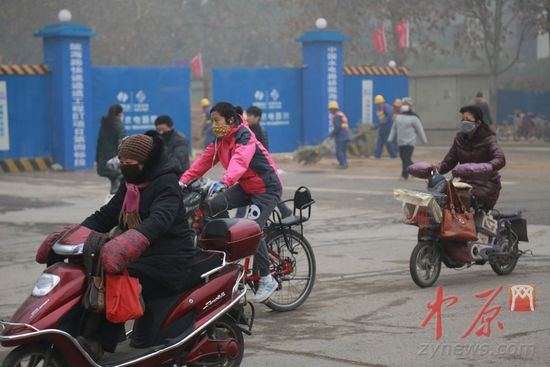
\includegraphics[width=\textwidth,height=2cm]{figures/1_1.jpg}}
          % 加入对这列的图片说明
		\centerline{交通}
	\end{minipage}
	\begin{minipage}{0.32\linewidth}
		\vspace{3pt}
		\centerline{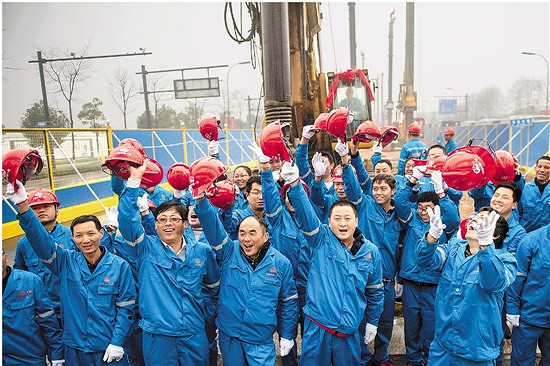
\includegraphics[width=\textwidth,height=2cm]{figures/1_2.jpg}}
	 
		\centerline{工地}
	\end{minipage}
	\begin{minipage}{0.32\linewidth}
		\vspace{3pt}
		\centerline{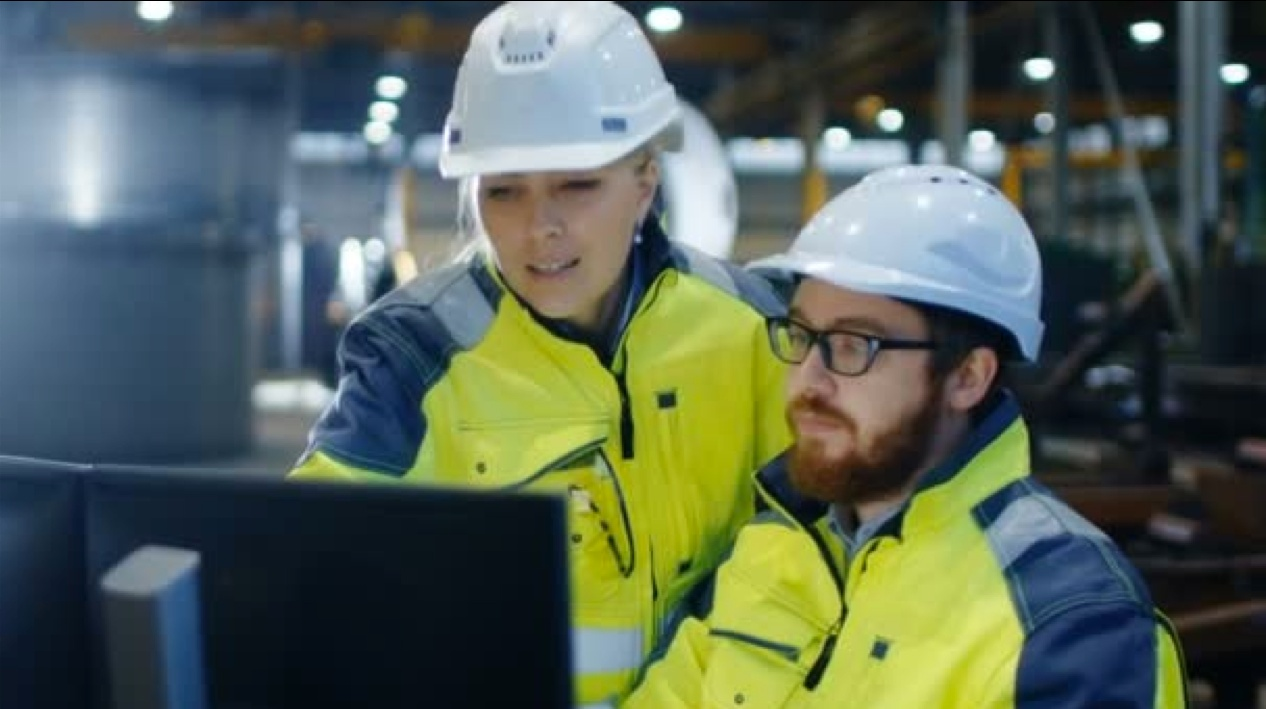
\includegraphics[width=\textwidth,height=2cm]{figures/1_3.jpg}}
	 
		\centerline{监测}
	\end{minipage}
 
	\caption{头盔在不同场景中的应用}
	\label{fig4}
\end{figure}

尽管许多国家和地区已经实施了强制佩戴头盔的法规,但在实际交通环境中,骑行者是否佩戴头盔并未得到有效监控。传统的人工检查方法存在效率低、准确性差等缺陷,难以满足现代城市交通管理的需求。因此,迫切需要一种高效、准确的技术手段来进行实时监测。
%1.1.2研究意义
\subsubsection{研究意义}

提升交通安全。通过对电动车骑行者头盔佩戴情况的实时检测,可以有效减少因未佩戴头盔而导致的交通事故伤亡。该技术能够帮助交通管理部门及时发现并纠正不安全行为,提升骑行者的安全防护意识,从而降低交通事故发生率,保护骑行者的生命安全。\par
广泛智能应用。本研究通过采用YOLOv8模型,将深度学习和计算机视觉技术应用于电动车头盔检测,展现了人工智能在交通安全管理中的前沿应用。该技术不仅实现了实时目标检测,还能够处理复杂的交通场景,极大地提升了检测的准确性和效率。这一创新的科技应用为未来更多智能交通解决方案的开发奠定了基础,推动了人工智能技术在公共安全领域的广泛应用。\par
提高安全意识。电动车头盔检测技术的推广应用,不仅能够直接改善交通安全状况,还能在公众中引发对安全骑行的重视。通过宣传和技术应用的结合,可以增强公众对佩戴头盔重要性的认识,逐步形成安全骑行的社会文化氛围,从而促进交通安全的全面提升。\par

%1.2研究问题分析
\subsection{研究问题分析}
YOLOv8(You Only Look Once Version 8)作为YOLO系列目标检测算法的最新版本,在处理电动车骑行者头盔检测等实际应用中展现出了巨大的潜力。它基于深度学习技术,通过优化的卷积神经网络架构,能够实现快速且准确的物体检测。这种轻量化设计使得YOLOv8能够在各种设备上高效运行,适合在交通监控系统中部署。该模型在复杂背景和不同光照条件下,仍能保持良好的检测性能,有助于及时识别未佩戴头盔的骑行者,从而为交通管理部门提供实时反馈和干预。\par
此外,YOLOv8的多任务处理能力,使其不仅限于目标检测,还可以应用于图像分割和关键点检测,进一步增强了其在智能交通系统中的应用价值。通过与交通管理系统的集成,YOLOv8能够有效提升城市交通管理的智能化水平,降低事故发生率,最终保护骑行者的生命安全。因此,YOLOv8的开发与应用,不仅推动了目标检测技术的发展,也为应对当前电动车安全隐患提供了切实可行的解决方案。
%2 引言
\section{行人数据图像处理}
%2.1 实验数据集
\subsection{实验数据集}
通过构建自定义数据集的方式,系统地收集了行人图像,共计纳入了7581张图片,其中训练集包含5457张图像,测试集包含1517张图像,验证集包含607张图像。该数据集涵盖了多种环境场景,如交通枢纽、建筑工地和制造车间等,旨在提升数据的多样性,进而增强模型的泛化能力。\par

\begin{figure}[h]
	
	\begin{minipage}{0.32\linewidth}
		\vspace{3pt}
        %这个图片路径替换成你的图片路径即可使用
		\centerline{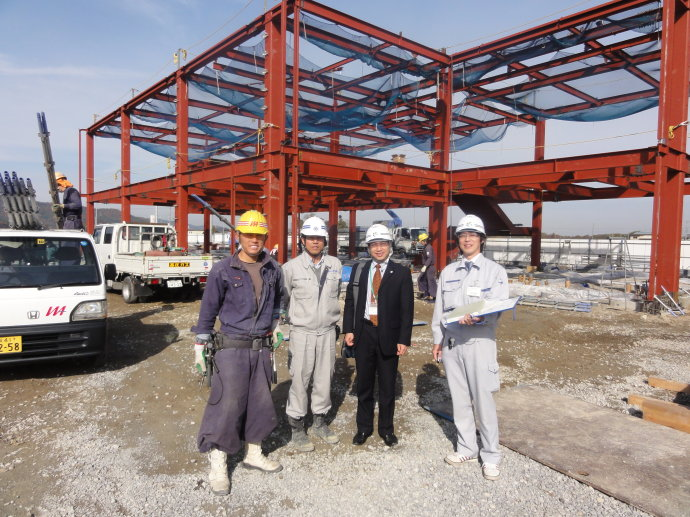
\includegraphics[width=\textwidth,height=2.5cm]{figures/2_1.jpg}}
          % 加入对这列的图片说明
		\centerline{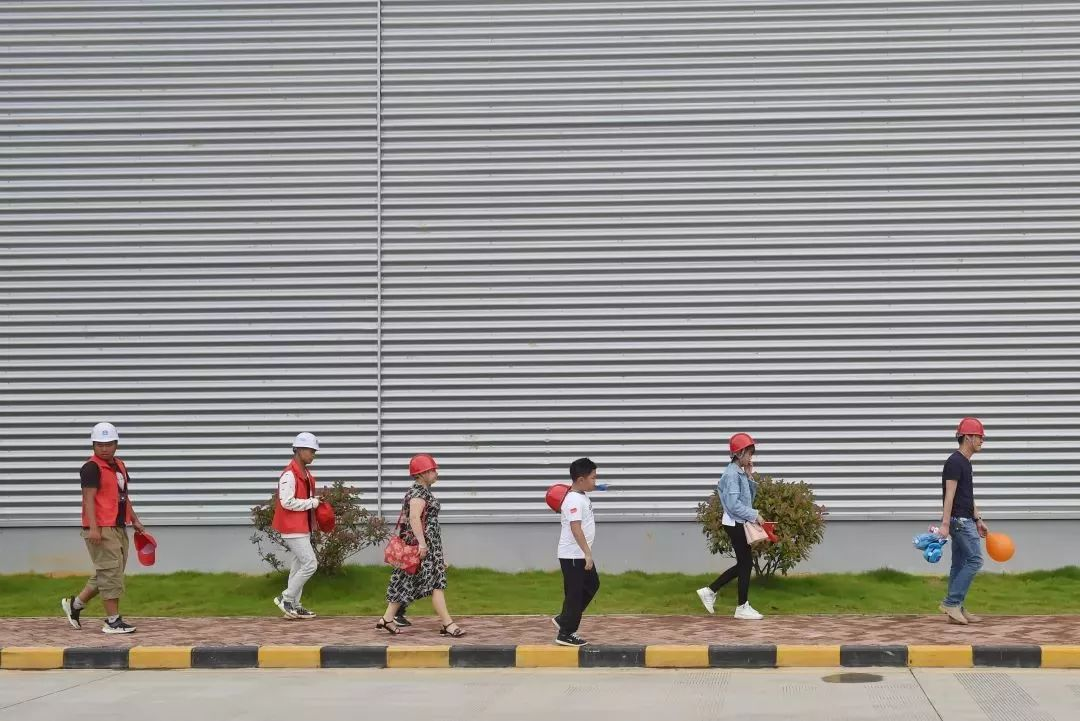
\includegraphics[width=\textwidth,height=2.5cm]{figures/2_2.jpg}}
	\end{minipage}
	\begin{minipage}{0.32\linewidth}
		\vspace{3pt}
		\centerline{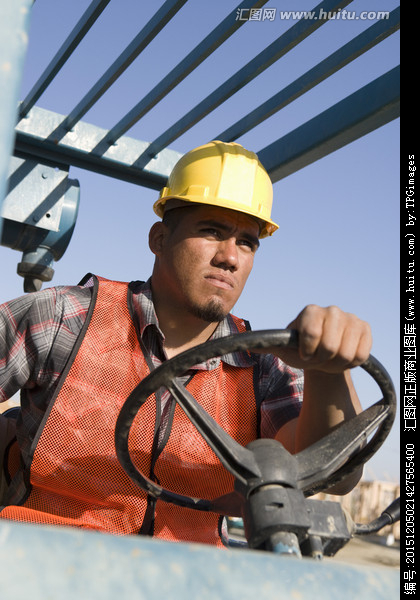
\includegraphics[width=\textwidth,height=2.5cm]{figures/2_3.jpg}}
	 
		\centerline{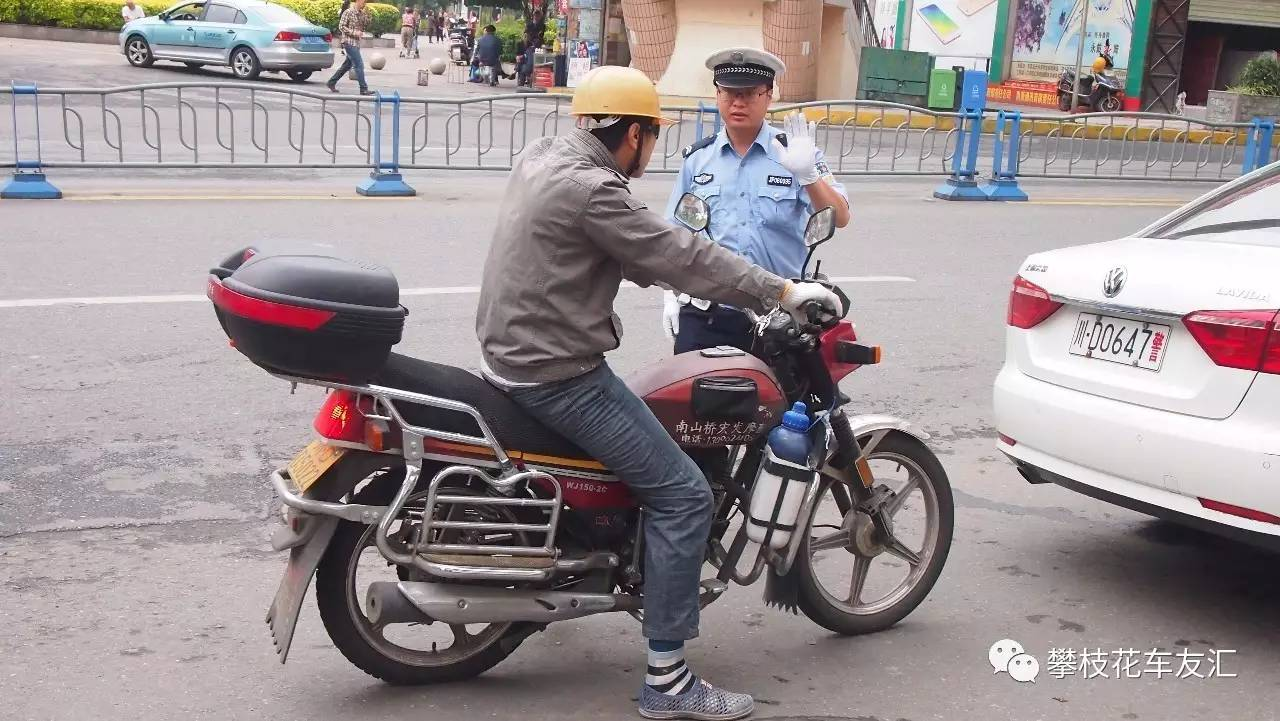
\includegraphics[width=\textwidth,height=2.5cm]{figures/2_4.jpg}}
	\end{minipage}
	\begin{minipage}{0.32\linewidth}
		\vspace{3pt}
		\centerline{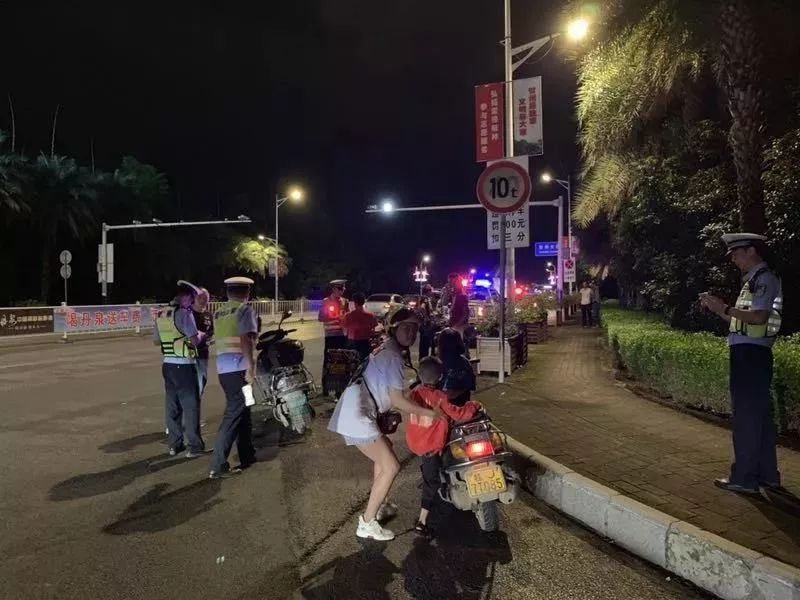
\includegraphics[width=\textwidth,height=2.5cm]{figures/2_5.jpg}}
	 
		\centerline{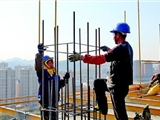
\includegraphics[width=\textwidth,height=2.5cm]{figures/2_6.jpg}}
	\end{minipage}
 
	\caption{多重环境下的行人数据图像}
	\label{fig4}
\end{figure}

在数据选择过程中,包含了多种实际环境下的图像样本,包括不同光照条件、背景复杂度及对象姿态的行人图像的收集,以确保各个类别样本的数量均衡。这种均衡性对于避免某一类别数据过多而导致的模型偏倚至关重要,从而确保模型能够在多种实际应用场景中展现出更高的适应性和鲁棒性。通过这种方法,旨在全面提升模型的性能,使其更好地适应复杂多变的环境。本研究将数据集划分为训练集、验证集和测试集,其中训练集占整体数据的80\%,验证集与测试集各占10\%。
%2.2 图像预处理
\subsection{图像预处理}
1)尺寸调整:为提高数据处理的效率,将所有图像尺寸调整为640×640像素。统一的图像尺寸能确保模型在训练和推理过程中能够获得一致的特征提取效果。\par
2)数据增广:为了增强数据集的多样性,并有效防止过拟合的发生,本文采用了随机旋转、翻转、裁剪及颜色调整等数据增广技术。通过数据增广生成更多的训练样本,提升模型对各种场景和条件的适应能力,从而提高模型泛化性能和鲁棒性。\par
3)归一化:在预处理最后阶段,进行像素值归一化,将其范围调整至0到1之间,从而有效减少因特征尺度差异带来的学习困难,提高训练效率,加快模型收敛速度并提升最终检测精度。
%2.3 yolo标准数据集
\subsection{YOLO标准数据集}
YOLO模型采用一种简单而高效的文本文件格式(.txt)进行对象数据的标注,每个图像对应一个标签文件。每一行代表一个物体,内容包括类别编号和边界框的坐标(归一化后的中心点 x, y 以及宽度和高度)。标签格式为:\textless class\textgreater, \textless x\_center\textgreater,\textless y\_center\textgreater,\textless width\textgreater,\textless height\textgreater,其中 class 是物体类别的编号,后四个参数分别表示边界框的中心坐标和宽高。
%2.4 数据集标注
\subsection{数据集标注}
本文在构建数据集时,选择YOLOv8模型作为基础,首先在小规模人工标注数据集上进行预训练,并通过迁移学习技术对模型进行微调,提升其对头盔检测任务的适应性。经过多次优化超参数以增强检测性能后,将训练完成的YOLOv8模型用于新图像数据的自动标注。通过模型推理,生成目标的边界框及相应的类别标签,成功识别佩戴头盔者和未佩戴头盔者,从而完成自动标注,大幅提高了标注效率,使生成时间较人工标注缩短约80\%。\par
\begin{figure}[htbp] 

   \centering
   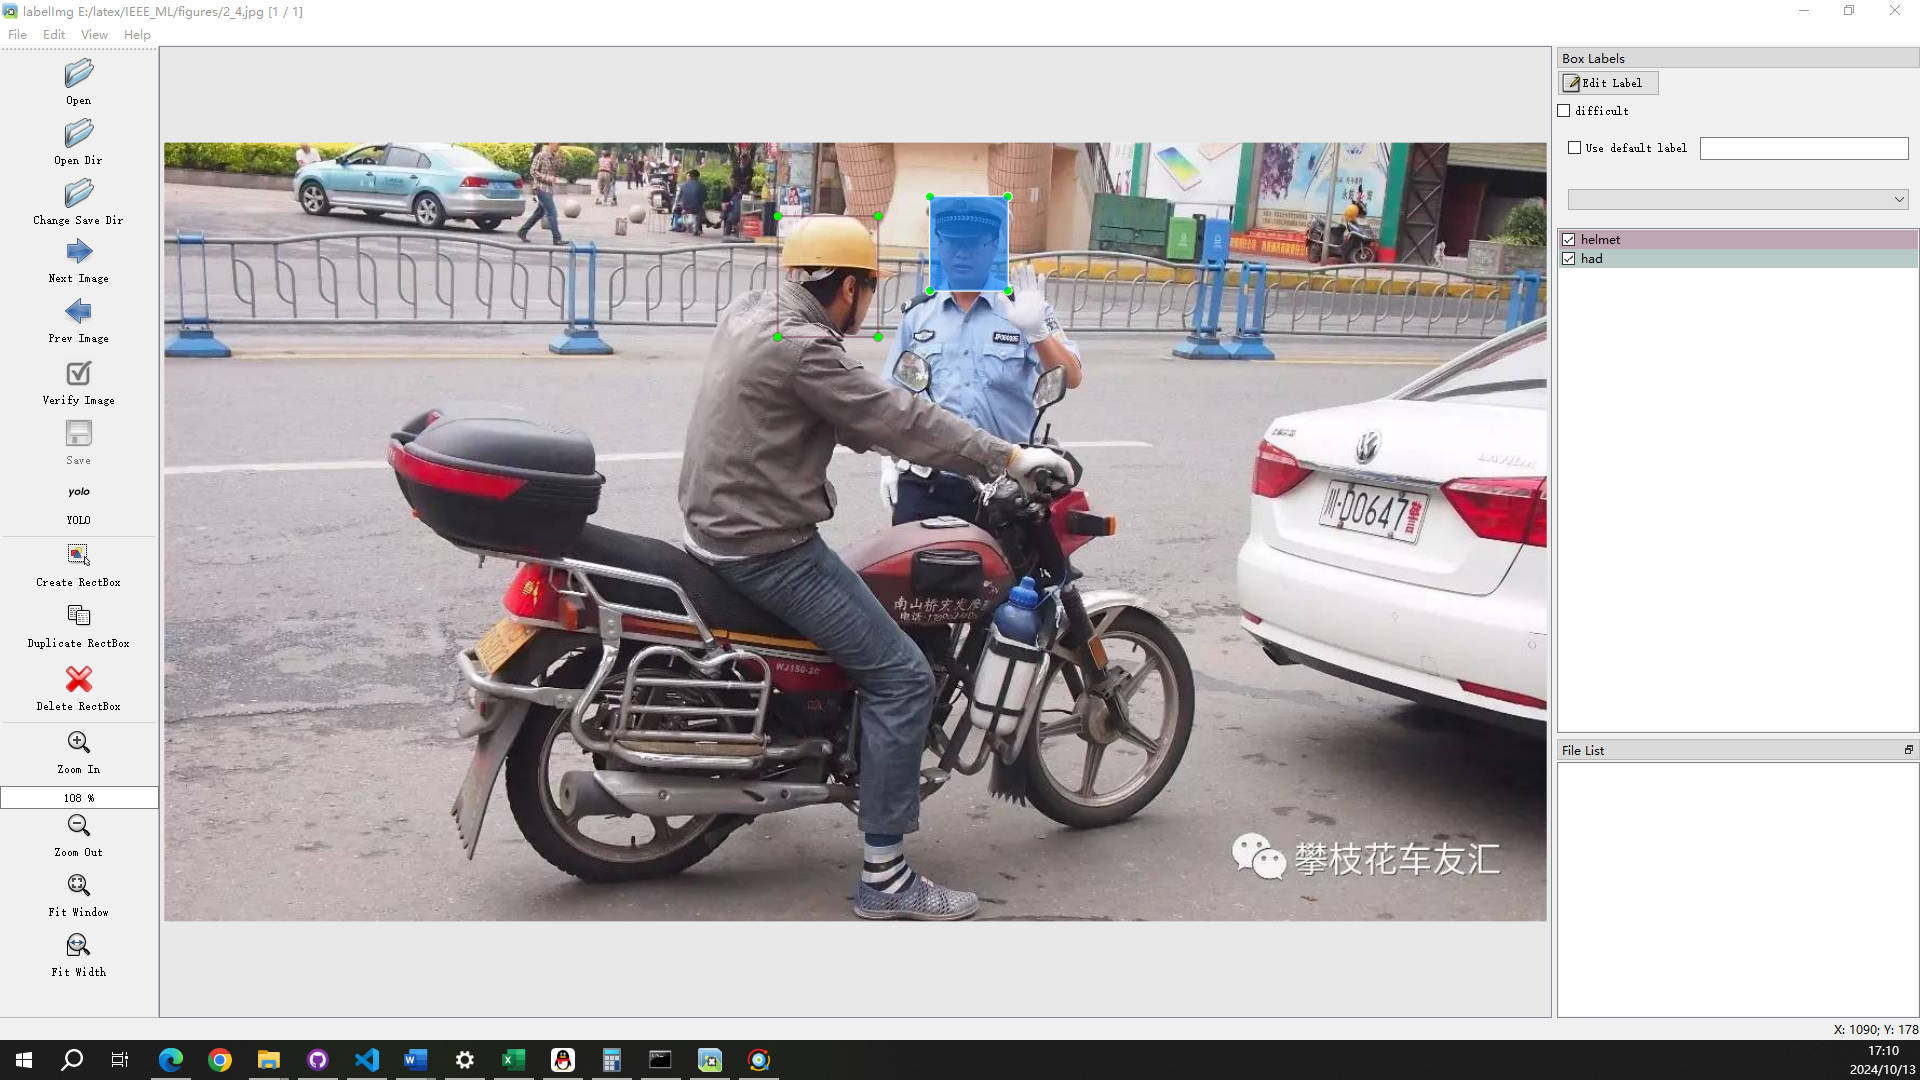
\includegraphics[width=3in,height=2in]{figures/2_7.jpg}
   \caption{标注后的数据} 
   \label{fig:} 
  
\end{figure} 
此外,为保证标注精度与可靠性,我们对照人工标注进行了比较分析和进行专家审查与修正,以强化标注数据的准确性和完整性。
%3 基于YOLOv8的检测系统实现
\section{基于YOLOv8的检测系统实现}
YOLOv8是一种精准高效的目标检测解决方案,系统采用YOLOv8作为核心检测算法,识别电动车及其驾驶员,并判断是否存在佩戴头盔行为。训练与测试使用的均为540*355的YOLO标准数据集,图3-1为整个实验流程图:
\begin{figure}[htbp] 

   \centering
   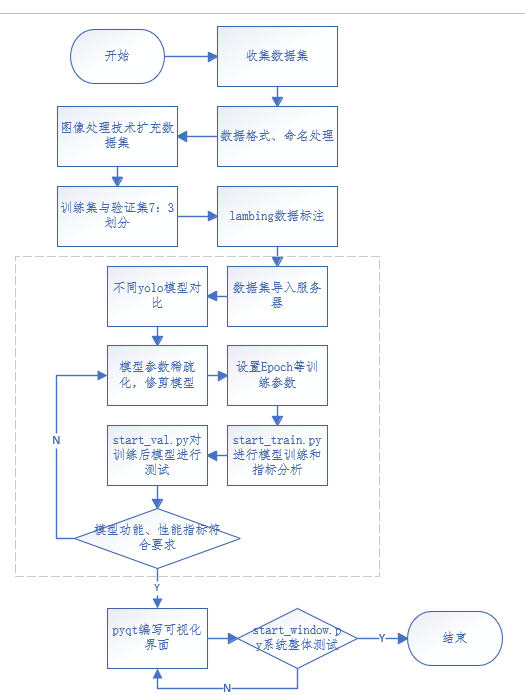
\includegraphics[width=2.5in]{figures/流程图.png}
   \caption{实验流程图} 
   \label{fig:} 
  
\end{figure} 

%3.1 训练环境搭建
\subsection{训练环境搭建}
对于大量图片数据集与复杂模型,通过GPU进行模型训练大加速,通过AutoDL平台租借云服务器实现YOLOv8模型的搭建,训练,测试与部署工作。\par
本次实验使用的硬件环境为:CPU 16 vCPU Intel(R) Xeon(R) Platinum 8481C,GPU RTX 4090D,显存大小24G,硬盘为80G。\par
软件环境:操作系统ubutnu22.04,编程语言python版本3.8.5,pytorch版本1.10.0,Cuda版本11.8。\par

%3.2 模型训练
\subsection{模型训练}
本次实验采用YOLOv8模型进行目标检测训练,整个训练过程依托于高性能服务器硬件及成熟的软件环境,确保了模型的高效收敛和稳定性能。\par
训练流程从数据准备开始,输入图像维度为像素540*355,首先对数据集进行了精细的标注、清洗和划分,形成训练集、验证集和测试集,为模型的训练和评估提供了坚实的数据基础。并且通过高性能硬件配置使得数据处理与模型计算可以高效并行执行,显著提高了训练效率。\par
整个训练过程共进行了100个epoch,训练阶段首先加载数据集,并进行数据增强操作,提高模型的泛化能力。接着初始化YOLOv8模型,设置包括学习率和批次大小等超参数,以确保训练初期能够有效学习特征。每个epoch包含前向传播、损失计算、反向传播和权重更新等步骤。\par
在服务器上,GPU的强大算力极大加速了这些运算,在卷积层的特征提取和参数更新过程中尤为显著。每个epoch结束后,模型会在验证集上进行评估,以监控性能并避免过拟合的发生。训练日志详细记录了每个epoch的损失、精度和召回率等关键指标,并且实时生成了损失曲线和精度曲线,以便于监控训练过程中的动态表现和分析模型的改进方向。\par
在进行模型参数配置时,为了确保对比实验的一致性和准确性,我们需要核心参数固定不变,以排除对训练效果产生的潜在影响。训练epoch为100轮,使用常见的随机梯度下降优化器,初始学习率和周期学习率均设置为0.01,设置batch数量为64。经训练,YOLOv8模型最终达到了预期的检测效果,能够精准地识别目标物体,表现出良好的鲁棒性和检测性能。通过数据预处理、模型初始化、迭代训练和模型评估的完整闭环与高性能服务器硬件的支持,使得模型在合理时间内完成了高效训练。\par

%3.3 模型部署
\subsection{模型部署}
在本项目中,我们将YOLOv8目标检测模型部署到基于PySide6开发的图形化界面应用中。模型部署的核心步骤包括开发UI界面,将经过训练的YOLOv8模型进行格式转换等。图3-2为UI界面。\par
\begin{figure}[htbp] 

   \centering
   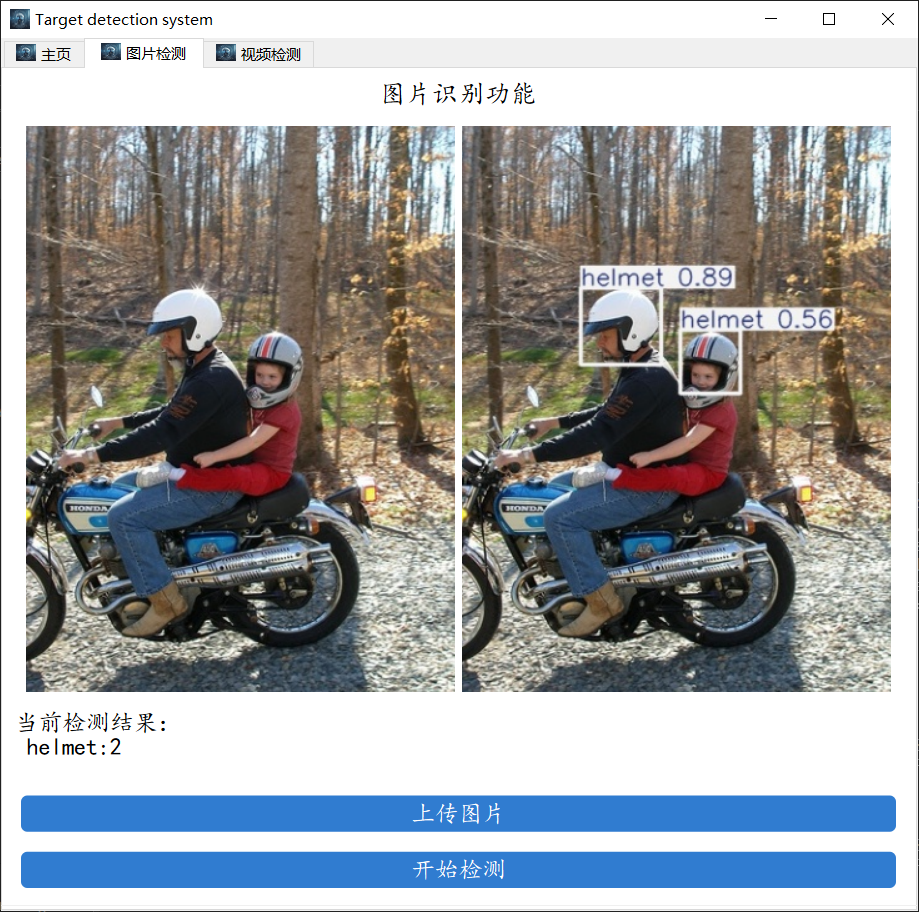
\includegraphics[width=2.5in]{figures/部署页面.png}
   \caption{部署界面} 
   \label{fig:} 
  
\end{figure} 
在应用程序中,用户能够通过直观的界面上传图像或视频流,并实时查看检测结果。这一过程中,我们充分利用了PySide6的强大功能,创建了用户友好的操作面板,使用户体验更加流畅。此外,部署过程中还进行了全面的测试,以确保在不同输入场景下的稳定性和可靠性。通过此次部署,YOLOv8模型得以在实际应用中发挥重要作用,推动了目标检测技术的实用化进程。\par


%4 调整与改进
\section{调整与改进}
电动自行车头盔的检测可能由于骑手的高速移动或环境的复杂性而变得颇具挑战性。例如,头盔可能因与摄像头距离较远而成为难以辨识的小目标。针对检测过程中低分辨率图像及小目标检测困难,背景与检测目标相似等问题,改进Yolov8n 模型。传统目标检测网络容易忽略或误判电动车骑行过程中远处、边缘或比例较小的头盔,进而导致漏检或误检。对此需要增强原始YOLOv8n模型以提升对小目标检测精度。\par
%4.1 
\subsection{卷积注意力模块}
本研究采用了基于卷积注意力机制模块(Convolutional Block Attention Module, CBAM)\textsuperscript{\cite{1}}的小目标检测优化策略。CBAM作为一种即插即用的注意力机制模块,可直接嵌入至多种流行的卷积神经网络架构中。该模块通过对输入特征图的不同区域赋予不同的权重,使网络能够更加聚焦于对特定任务具有重要性的信息,同时忽略不相关的信息。因此,在针对佩戴头盔的行人检测任务中,由于目标与摄像头距离较远导致行人及头盔尺寸较小,且在检测图像中所占比例较低,引入CBAM能够使网络更加专注于前景中的小目标,并有效定位感兴趣的区域。这进一步增强了网络的特征提取能力,使得在最小感受野的特征图上能够更精确地识别小目标。CBAM的总体架构如图\Ref{fig:CBAM}所示。\par

\begin{figure}
  \centering
  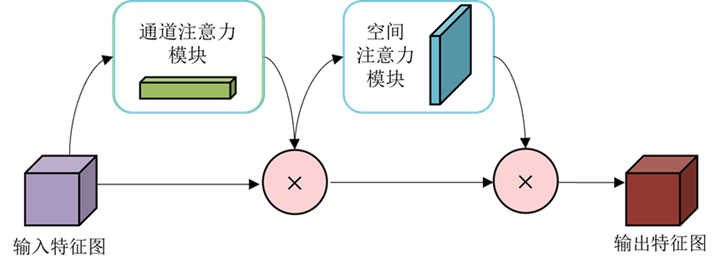
\includegraphics[width=2.5in]{./figures/4_1.png}
  \caption{CBAM结构图}
  \label{fig:CBAM}
\end{figure}

对于输入特征图$X\in R^{c\times h\times w}$ ,CBAM先使用通道注意力模块,在宽高维度上对输入进行平均池化和最大池化的操作,得到两个$c\times1\times1$大小的张量。然后,将两个张量分别经过共享卷积层,将输出进行逐元素相加,再经过非线性激活操作,得到通道注意力权值,即大小为$c\times1\times1$的张量。将该权值与输入特征图进行逐元素相乘,得到通道注意力模块的输出特征图$X^{\prime}\in R^{c\times h\times w}$ 。接着,对于通道注意力模块的输出特征图,在通道维度上进行平均池化和最大池化操作,得到两个$1\times h\times w$大小的张量。然后,将两个张量在通道维度上进行拼接,并经过一个卷积操作,将通道维度降为1。最终,经过非线性激活操作,得到空间注意力权值,即大小为$1\times h\times w$的张量。将该权值与通道注意力模块的输出特征图进行逐元素相乘,便得到经过卷积注意力模块处理后的输出特征图。根据论文[1]中的实验结果,在不同的图像分类和目标检测数据集上,将CBAM集成到不同的神经网络模型中后,模型的性能得到很大的提高,这证明了该模块的有效性。\par

针对YOLOv8n网络,本文将卷积注意力CBAM模块应用在了特征金字塔网络下采样过程中的每一个跨阶段局部模块之后,对不同层次的特征进行融合的Neck部分,模型框架修改后如图\ref{fig:Neck}所示。\par

\begin{figure}
  \centering
  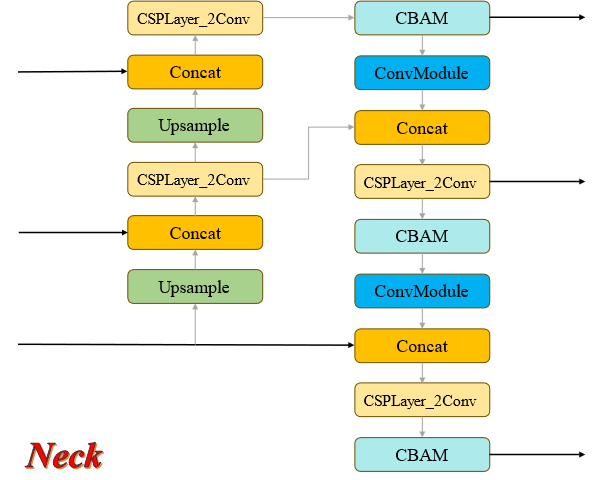
\includegraphics[width=2.5in]{./figures/4_2.png}
  \caption{应用CBAM卷积注意力模块网络Neck部分结构图}
  \label{fig:Neck}
\end{figure}

%4.2 
\subsection{Transformer Block}
Transformer\textsuperscript{\cite{2}}是一种专为处理序列数据而设计的深度学习架构。该模型利用自注意力机制实现了高效的并行计算,并具备捕获长距离依赖关系的能力。\par

\begin{figure}
  \centering
  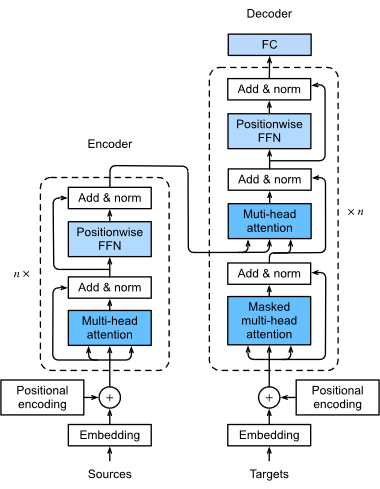
\includegraphics[width=2.5in]{./figures/4_3.png}
  \caption{Transformer结构图}
  \label{fig:Transformer}
\end{figure}

Transformer的结构如图\ref{fig:Transformer}所示,主要由编码器和解码器两大部分构成。编码器负责将输入信息映射为中间的隐藏状态表示,而解码器则将这些隐藏状态转换为最终的输出序列。编码器由若干相同的编码器层堆叠而成,每一层均包含自注意力机制和前馈神经网络。解码器在结构上与编码器相似,但额外增加了一个注意力层,该层用于关注编码器的输出。\par

多头自注意力机制是Transformer的核心,它使得模型在处理输入序列时能够同时关注序列中不同位置的信息。查询、键和值通过不同的线性变换分成多组(头),然后对每组进行自注意力计算,最后将所有头的输出拼接起来,再次通过一个线性层得到最终的输出。\par

前馈网络是注意力机制之后的一个关键组件。对注意力层的输出进行进一步的非线性变换,以捕获更复杂的特征和表示。\par

\begin{figure}
  \centering
  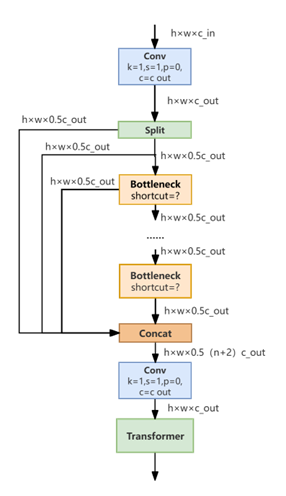
\includegraphics[width=2.5in]{./figures/4_4.png}
  \caption{添加Transformer后的C2f结构图}
  \label{fig:C2fr}
\end{figure}

针对YOLOv8n网络,本文在特征处理的中间层C2f中加入Transformer模块,修改后的C2f结构如图\ref{fig:C2fr}所示。通过引入自注意力机制,修改后的模型能够更好地捕捉长距离依赖关系,这有助于模型在处理图像时能够更好地理解全局上下文信息,从而提升特征的表示能力。且由于Transformer block能够有效捕捉全局信息,从而帮助模型在不同的尺度上捕捉到小目标的特征,能够更好地区分头盔与复杂的背景。此外,在YOLOv8n的架构中,特征融合是一个关键环节。Transformer block可以作为一种有效的特征融合工具,通过自注意力机制融合不同层次的特征信息,提高模型在各种环境下的鲁棒性,减少误报和漏报,进一步提升检测性能。


%5 实验结果
\section{实验结果}
The conclusion goes here.

%6 总结与展望
\section{总结与展望}
本文针对人员头盔佩戴检测中面临的诸多挑战,提出了一种基于YOLOv8模型的改进方法。当前检测技术在处理精度不足、小目标和被遮挡目标的误检与漏检现象,以及检测过程的高耗时和复杂性等方面存在显著问题。为了解决这些问题,本文在YOLOv8模型的基础上进行优化,首先用Transformer block替换了c2f中的bottle neck,增强了模型对复杂场景中目标特征的提取能力,同时在特征提取过程中融入了CBAM模块,进一步提升了模型对重点区域的关注度和整体检测精度。改进后的模型显著提高了头盔佩戴检测的准确率和检测效率,实验结果表明,该模型能够很好地应对交通场景中头盔检测任务的实际需求。\par
此外,改进的YOLOv8模型在实现高精度检测的同时,依然保持了轻量化的优势,确保其在实际应用中的广泛性和便捷性。通过优化主干网络结构以及整合高效的上采样技术,该模型不仅能有效地处理小目标和被遮挡目标,还能够应对复杂背景下的干扰,一定程度的减少误检的发生率。这使得该模型在协助交警和相关执法部门进行自动化执法时具有较大的潜力,能够提高对未佩戴头盔等交通违规行为的检测和查处效率,进而保障交通安全。\par
然而,尽管改进后的YOLOv8模型展示出了优异的综合性能,仍然存在一些不足。特别是在极端环境条件下,被遮挡目标的检测效果仍有提升空间。因此,未来的研究将进一步考虑采用DETR系列等更先进的神经网络架构和训练策略,以提升模型的鲁棒性和泛化能力。此外对于特定场景,如强光环境或雷雨天气下会出现一定的检测误差,在后续的研究中,会着眼于多种实际场景下的应用,引入迁移学习,提升模型的泛化性。


% if have a single appendix:
%\appendix[Proof of the Zonklar Equations]
% or
%\appendix  % for no appendix heading
% do not use \section anymore after \appendix, only \section*
% is possibly needed

% use appendices with more than one appendix
% then use \section to start each appendix
% you must declare a \section before using any
% \subsection or using \label (\appendices by itself
% starts a section numbered zero.)
%

% use section* for acknowledgment
\section*{致谢}


The authors would like to thank...


% Can use something like this to put references on a page
% by themselves when using endfloat and the captionsoff option.
\ifCLASSOPTIONcaptionsoff
  \newpage
\fi



% 参考文献
\begin{thebibliography}{1}

\bibitem{1}
Woo S, Park J, Lee J Y, et al. CBAM: Convolutional block attention module[C]//Proceedings of the European conference on computer vision (ECCV). 2018: 3-19.

\bibitem{2}
Vaswani A. Attention is all you need[J]. Advances in Neural Information Processing Systems, 2017.

\end{thebibliography}


% that's all folks
\end{document}


